% !TEX root = ../ORM_report.tex
\section{Цель работы}
Получить практические навыки работы с БД через механизм объектно-реляционного отображения.

\section{Программа работы}
\begin{enumerate}
	\item Знакомство с фреймворком Django:
	\begin{itemize}
		\item установка;
		\item создание проекта;
		\item создание приложения;
	\end{itemize}
	\item  Формирование набора моделей, соответствующих схеме БД, полученной по результатам разработки схемы БД и модификации схемы;
	\item Знакомство с механизмом миграций: автоматическое формирование схемы БД с помощью миграций;
	\item Создание manage-команд для заполнения БД тестовыми данными (по несколько записей в каждой таблице);
	\item Написание отчета.
\end{enumerate}

\section{Ход работы}
\subsection{Подготовка}
Предварительно был установлен следующий комплекс программ:

\begin{itemize}
\item Python 3.6;
\item PostgreSQL 9.6.2;
\item Psycopg 2.6.2;
\item Django 1.10.5.
\end{itemize}

Для PostgreSQL была создана база данных \textbf{mus}, а также пользователь \textbf{dan0n}.
Далее следующими командами был создан проект:

\begin{lstlisting}[caption=Создание проекта]
D:\4 course\lastsem\db\lab1>django-admin.py startproject lab1
D:\4 course\lastsem\db\lab1>cd lab1
D:\4 course\lastsem\db\lab1\lab1>python manage.py startapp mus
\end{lstlisting}

Для изменения стандартных настроек был открыт файл ...lab1$\backslash$lab1$\backslash$lab1$\backslash$settings.py. Первоначально в нем содержались следующие строчки:

\begin{lstlisting}[caption=Часть settings.py до изменений]
...

DATABASES = {
	'default': {
		'ENGINE': 'django.db.backends.sqlite3',
		'NAME': os.path.join(BASE_DIR, 'db.sqlite3'),
	}
}

...

INSTALLED_APPS = [
	'django.contrib.admin',
	'django.contrib.auth',
	'django.contrib.contenttypes',
	'django.contrib.sessions',
	'django.contrib.messages',
	'django.contrib.staticfiles',
]

...
\end{lstlisting}

Они были заменены на следующие:

\begin{lstlisting}[caption=Часть settings.py после изменений]
...

DATABASES = {
	'default': {
		'ENGINE': 'django.db.backends.postgresql_psycopg2',
		'NAME': 'mus',
		'USER': 'dan0n',
		'PASSWORD': 'myasnov',
		'HOST': 'localhost',
		'PORT': '5432',
	}
}

...

INSTALLED_APPS = [
	'django.contrib.admin',
	'django.contrib.auth',
	'django.contrib.contenttypes',
	'django.contrib.sessions',
	'django.contrib.messages',
	'django.contrib.staticfiles',
	'mus',
]

...
\end{lstlisting}

Далее, для формирования моделей необходимо открыть файл ...lab1$\backslash$lab1$\backslash$mus$\backslash$models.py. В данном файле описываются модели для последующей миграции.

\subsection{Миграция}
По результатам прошлых лабораторных работ имеется схема БД, приведенная на \vref{fig:db_scheme}, согласно которой будут формироваться соответствующие модели для миграции.

\begin{figure}[H]
	\centering
	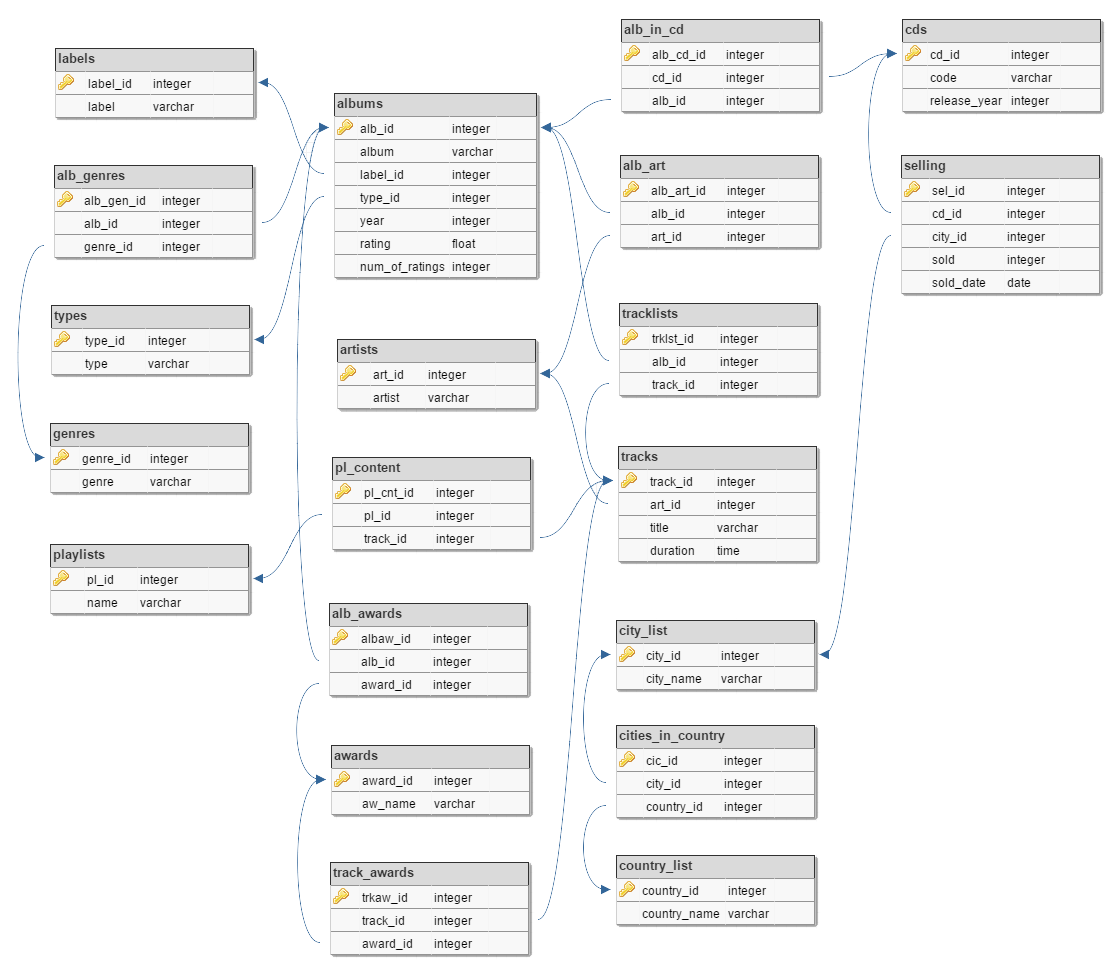
\includegraphics[width=0.95\textwidth]{scheme_m}
	\caption{SQL-схема БД}
	\label{fig:db_scheme}
\end{figure}

В файл models.py были добавлены модели, соответствующие приведенной базе данных.

\lstinputlisting[caption=models.py]{code/models.py}

Если ключ является вторичным, то Django автоматически допишет \textbf{\_id} к данному полю. Также необходимо указывать класс Meta для каждой таблицы, иначе Django автоматически допишет название проекта к каждой таблице. К тому же необязательно самостоятельно указывать первичные ключи, т.к. Django добавит их автоматически при отсутствии.

После написания моделей был запущен процесс миграции.

\begin{lstlisting}[caption=Процесс миграция]
D:\4 course\lastsem\db\lab1\lab1>python manage.py makemigrations mus
Migrations for 'mus':
  mus\migrations\0001_initial.py:
    - Create model AlbArt
    - Create model AlbAwards
    - Create model AlbGenres
    - Create model AlbInCd
    - Create model Albums
    - Create model Artists
    - Create model Awards
    - Create model Cds
    - Create model CitiesInCountry
    - Create model CityList
    - Create model CountryList
    - Create model Genres
    - Create model Labels
    - Create model Playlists
    - Create model PlContent
    - Create model Selling
    - Create model TrackAwards
    - Create model Tracklists
    - Create model Tracks
    - Create model Types
    - Add field track to tracklists
    - Add field track to trackawards
    - Add field track to plcontent
    - Add field city to citiesincountry
    - Add field country to citiesincountry
    - Add field label to albums
    - Add field type to albums
    - Add field alb to albincd
    - Add field cd to albincd
    - Add field alb to albgenres
    - Add field genre to albgenres
    - Add field alb to albawards
    - Add field award to albawards
    - Add field alb to albart
    - Add field art to albart

D:\4 course\lastsem\db\lab1\lab1>python manage.py migrate mus
Operations to perform:
Apply all migrations: mus
Running migrations:
Applying mus.0001_initial... OK
\end{lstlisting}

По завершении миграции база данных содержит все таблицы из схемы, а также таблицу \textbf{django\_migrations}, которая необходима для работы системы миграции Django.

\subsection{Manage-команды}
Для реализации manage-команд по заполнению базы данных, в директорию проекта \textbf{mus} была добавлена директория \textbf{management} и сопутствующие файлы. Дерево директории mus теперь выглядит следующим образом:

\dirtree{%
	.1 mus.
	.2 admin.py.
	.2 \_\_init\_\_.py.
	.2 management.
	.3 commands.
	.4 \_\_init\_\_.py.
	.4 populate\_db.py.
	.3 \_\_init\_\_.py.
	.2 models.py.
	.2 прочие файлы.
}

Файл \textbf{populate\_db.py} отвечает за исполнение команд. Для заполнения каждой таблицы 3 значениями, в данный файл были внесены соответствующие команды.

\lstinputlisting[caption=populate\_db.py]{code/populate_db.py}

Теперь запустим команду и проверим с помощью psql.

\begin{lstlisting}[caption=Выполнение manage-команды]
D:\4 course\lastsem\db\lab1\lab1>python manage.py populate_db

D:\4 course\lastsem\db\lab1\lab1>psql -U postgres
Пароль пользователя postgres:
psql (9.6.2)
Введите "help", чтобы получить справку.

postgres=# \c mus
Вы подключены к базе данных "mus" как пользователь "postgres".
mus=# SELECT * FROM Tracks;
 track_id |    title    | duration | art_id
----------+-------------+----------+--------
        1 | Jailbreak   | 00:04:48 |      1
        2 | Do It Right | 00:05:33 |      2
        3 | Killer Bee  | 00:04:20 |      3
\end{lstlisting}

 Как и ожидалось, данные были успешно добавлены в БД.

\section{Вывод}
В результате работы было проведено знакомство с миграциями моделей на примере Django, а также с manage-командами для заполнения БД.

К достоинствам миграции Django можно отнести:
\begin{itemize}
	\item Отслеживание схемы БД;
	\item Поддержка различных БД (PostgreSQL, MySQL, SQLite);
	\item Ускорение процесса изменения схемы базы данных;
	\item Возможность отката изменений.
\end{itemize}

К недостаткам можно отнести переход от стандартизированных sql запросов и команд к собственному формату Django, что требует некоторого изучения перед использованием.

Также был проведен опыт использования manage-команд. Использование данного инструмента позволяет расширить проект собственными командами, к примеру, геератором псевдослучайных записей в БД.